\section{L\"osung Pflichtimplementierung}
\label{sec:lsgpflicht}

Wie bereits im Abschnitt "`Aufgabenstellung"' beschrieben, war es Gegenstand der Pflichtimplementierung, dass das Auto autonom mittels Sensorik fahren kann, die Kamera ArUco-Marker erkennt, sowie das Auto durch ein Tor aus solchen hindurchfahren kann. Bereits in obigem Abschnitt wurden die Rahmenbedingungen, welche wir für unsere Lösung angenommen haben definiert. Im Folgenden wird nun erläutert, wie wir, auf Grundlage des Zustandsautomaten, dessen genaue Implementierung erst später erläutert wird, die drei Hauptaufgaben realisiert haben.

%%%%%%
\subsection{Autonomes Fahren}
Unser Konzept zum autonomen Fahren baut sehr stark auf den Möglichkeiten, die uns eine FSM (Finite State Machine/Zustandsautomat) bietet, auf. 
Das Konzept beruht grundlegend darauf, dass das Auto eine FSM lädt, die entweder per JSON-File (genaueres zu JSON, s. Abschnitt 8) oder per graphischer Oberfläche (genaueres zur graphischen Programmierung, s. Abschnitt 9) konfiguriert wird. Die FSM ist ein Graph aus verschiedenen Zuständen, die jeweils eine Funktion des Autos, wie z.B. geradeaus an einer Wand entlang fahren, repräsentieren. Diese verschiedenen Funktionen oder Zustände des Autos sind über Transitionen verbunden, d.h. Ereignisse, die zu einem Zustandswechsel führen. Das kann z.B. eine abrupte Abstandsänderung der führenden Wand sein.
\newline 
Mittels der Kombination aus Zuständen, in denen sich das Auto befinden kann und Ereignissen, die zu einem Zustandswechsel führen, kann ein autonomen Verhalten, je nach Umgebung des Autos realisiert werden. Alternativ kann ein Weg in einem Bekannten Umfeld einprogrammiert werden, indem eine Folge von Zuständen konkateniert wird. 
Der Basiszustand für das autonome Fahren ist ein einfacher Wandfolger-Zustand, der das geregelte Geradeausfahren entlang einer Wand realisiert. 
\newline
\newline
Ein Regelkreis sorgt dafür, dass ein System in einen stabilen Zustand überführt wird. Dazu wird eine Eingangsgröße, in diesem Fall der Abstand zur Wand, in einen Regelkreis geführt. Ausgangsgröße ist dann der Lenkeinschlag, welcher den Abstand des Autos zur Wand beeinflusst. Um nun den Wandabstand stabil zu halten, wird die Differenz zwischen der Regelgröße (Lenkeinschlag) und Führungsgröße (Wandabstand) bestimmt (Regelabweichung). Da die einzelnen Regelkreisglieder ein Zeitverhalten haben, muss der Regler den Wert der Abweichung verstärken, sowie das Zeitverhalten unterdrücken. 
Anfangs haben wir versucht, das Regelverhalten durch einen PID-Regler abzubilden, jedoch führten Tests und Hinweise der Gruppe \textit{Nullpointer} des vergangenen Semesters zu einer Vernachlässigung des I-Anteils. Generell sorgt der P-Anteil für eine proportionale Verstärkung der Regelabweichung. Der D-Anteil sorgt für ein differenzierendes Verhalten, ist also abhängig von der Änderungsgeschwindigkeit der Regelabweichung.
Der vernachlässigte I-Anteil sorgt für eine zeitliche Integration der Regelabweichung. Dies führt bei dem Auto zu einer sich mit höherem I-Anteil einstellenden Trägheit, die das Auto unflexibler macht.

Der Basiscode, mit dem der Regler implementiert wird, ist in der Klasse \textit{BasicFollowWall} (Zeile 53) zu sehen:
\begin{lstlisting}
double y = _p * e + _esum * _i * PID_S + _d * (e - _eold)*PID_INVS;
\end{lstlisting}

Hierbei stellen \textit{PID\_S} und \textit{PID\_INVS} Konstanten dar (0.0125 und 80). \textit{\_p} ist der Proportionalanteil, \textit{\_i} der Integralanteil und \textit{\_d} der Differentialanteil. e ist die Eingangsgröße, \textit{\_esum} die aufaddierten Wandabstände der vergangenen Durchläufe und \textit{\_eold} der Wert des letzten Durchlaufes. \textit{y} ist der daraus berechnete Lenkeinschlag.
\newline
\newline
Mittels des oben vorgestellten PD-Reglers wird im Zustand \textit{BasicFollowWall} das Geradeausfahren implementiert. Erste Tests haben gezeigt, das entgegen der Erwartungen auch Kurven mit dem gleichen Zustand umfahren werden konnten. Daraus ergab sich dann die Einsicht, dass kein neuer Kurvenzustand eingeführt werden musste. Es lassen sich also alle grundlegenden Bewegungen durch eine Konkatenation verschieden parametrisierter Wall-Follow Zustände erreichen. Zudem hat sich herausgestellt, dass Kurven umso besser funktionieren, wenn unmittelbar vorher die Geschwindigkeit gedrosselt wird und im Anschluss ein größerer Wandabstand gewählt wird, da sonst die Gefahr besteht, dass die Ultraschallsensoren einen zu steilen Winkel zur Wand haben. 
Nun ist es also möglich mit einem einzigen Zustand (BasicFollowWall) die grundlegenden Bewegungen (Geradeausfahren, Kurvenfahren) abzudecken. Als Transitionen zwischen den Zuständen haben wir vier Optionen implementiert: \textit{Always, Distance, Finished, SensorLevel}. 
\begin{itemize}
	\item \textbf{Always}: Diese Transition feuert sofort.
	\item \textbf{Distance}: Diese Transition feuert nach der übergebenen Distanz. Die aktuelle Distanz wird immer über die Hall-Sensoren aus dem aktuellen Maschinen-Zustand (Machine State) ausgelesen. 
	\item \textbf{Finished}: Um zu feuern, muss die Methode \textit{isFinished()} des vorangegangenen Zustands \textit{true} zurückgeben. Diese Transition ist also nur möglich, wenn der vorige Zustand das Interface \textit{IFinishable} implementiert. 
	\item \textbf{SensorLevel}:	SensorLevel ist die meistgenutzte Transition. Sie feuert immer dann, wenn ein vorgegebener Sensorwert über oder unterschritten wurde. Diese Transition kann Werte aller drei Ultraschallsensoren als Referenz nehmen und sowohl bei Über- oder Unterschreiten eines Grenzwertes aktiv werden. 
\end{itemize}
Neben dem BasicFollowWall-State sind noch einige weitere States implementiert, die jeweils spezielle Aufgaben erfüllen und im Folgenden knapp vorgestellt werden:
\begin{itemize}
	\item \textbf{ApproachPoint}: Es kann ein Punkt übergeben werden, der dann geregelt angefahren wird. Dieser Zustand wurde von uns dafür erstellt, einen Punkt einen Meter vor einem ArUco-Tor anzufahren.
	\item \textbf{ArucoGateCenter}: Dieser Zustand richtet das Auto aus, wenn es vor einem ArUco-Tor steht, um das Tor anschließend gerade zu durchfahren. Dies ist nötig, da das Auto nach Transition aus dem ApproachPoint-Zustand nicht rechtwinklig zur Verbindungsgeraden der beiden Marker-Mittelpunkte ausgerichtet ist.
	\item \textbf{FollowWall}: FollowWall ist eine Modifikation des BasicFollowWall-Zustandes. Ziel war, dass die Regelung Türrahmen ignoriert, sodass sich das Auto anschließend nicht stark aufschaukelt. Dies wurden erreicht, indem Abweichungen der Ultraschallsensorwerte, die größer als 2cm sind, ignoriert werden. Dies bringt den Vorteil mit sich, dass das Auto sehr stabil gerade aus fährt. Nachteilig ist jedoch, dass es nicht mehr oder nur noch sehr schwach auf größere Änderungen der Umgebung reagiert. Zur Erkennung von Kurven ist dies jedoch kein Problem, da diese ja in der folgenden Transition getriggert werden.
	\item \textbf{FollowWallRamp}: Dieser Zustand ermöglicht eine Abstandsregelung zu einer das Auto umgebenden Wand nach einer linearen Funktion. Er ermöglicht somit z.B. einen Spurwechsel oder das Umfahren von Hindernissen.
	\item \textbf{FSMState}: Dieser Zustand ermöglicht das Einbinden von Zustandsautomaten als eigenen Zustand in einer FSM. Dies schafft eine sehr starke Abstraktion, sodass eine Zustandsfolge, z.B. zur Kurvenfahrt, abstrakt eingebunden werden kann und die Größe des Gesamtautomaten überschaubar bleibt.
	\item \textbf{Idle}: Dieser Zustand macht nichts. 
	\item \textbf{Motor}: Hier fährt das Auto einfach mit festgelegter Geschwindigkeit eine festgelegte Distanz geradeaus.
	\item \textbf{Stop}: Dieser Zustand stoppt das Auto.
\end{itemize}
Mittels der vorgestellten Konstrukte kann nun eine beliebige Abfolge von Aktivitäten des Autos abgebildet werden. Es ist möglich, ihm eine Strecke oder alternativ ein Verhalten einzuprogammieren. Ein autonomes Verhalten wird z.B. über mehrere parallele Zweige im Automaten realisiert. Als Beispiel fährt das Auto geradeaus und falls ein Hindernis auftritt, feuert eine Transition, die mehrere Zustände zu dessen Umfahren triggert. Werden Marker erkannt, könnte eine andere Transition feuern und je nach ID ein Verhalten des Autos auslösen.

Durch die vorgestellte Modularität ist das autonome Verhalten des Autos um (fast) beliebig Szenarien erweiterbar (Fliegen lernen wird es leider ohne Hardwareanpassungen nie können).
%%%%%%
\subsection{Erkennung ArUco-Marker}
Die Erkennung der ArUco-Marker ist durch einen ROS-Node implementiert. Dort haben wir zur Kamerakalibrierung eine Kombination der ROS-internen Kalibrierung und der Kalibrierung der  \textbf{OpenCV}\footnote[1]{http://opencv.org/} Open Source Software Bibliothek verwendet. Zur Kalibrierung wird ein Schachbrettmuster verwendet. Dabei übergibt man der OpenCV-Routine die Anzahl der Kästchen und deren Größe. Nachdem die Eckpunkte erkannt sind, werden verschiedene Orientierungen im Raum dargestellt, um eine robuste Kalibrierung zu erreichen. Anhand der Zuordnungen von Raum zu Bildkoordinaten kann nun die Kalibrierungsmatrix berechnet werden. 
OpenCV erkennt nun die ArUco-Marker und kann deren Position errechnen. Die Daten dazu werden anschließend in einer ROS-Topic gepublisht. Unserer Anwendungssoftware stehen so die genauen Bildkoordinaten der Marker und ihre Ausrichtung im Raum zur Verfügung.  

%%%%%%
\subsection{Durchfahren von Toren}
Nachdem nun dargestellt wurde, wie ArUco-Marker erkannt werden, bedarf es nur noch eines weiteren Schrittes, um das erkannte ArUco-Tor zu durchfahren. Man muss anhand der erhaltenen Koordinaten den weiteren Streckenverlauf so umplanen, dass das Tor durchfahren wird. 
\newline
Dazu gibt es verschiedene mögliche Ansätze. Zuerst war geplant, eine S-Kurve zu berechnen, deren Startpunkt die aktuelle Position und deren Endpunkt ein Punkt unmittelbar vor dem ArUco-Tor ist. Der Vorteil dieser Implementierung ist, dass das Auto vor dem Tor schon senkrecht zur Verbindungsstrecke der beiden Markermittelpunkte ausgerichtet ist, sodass es dann nur noch geradeaus fahren muss. Dazu war es nötig, sowohl Kenntnis über die Strecke, welche durch eine Hallsensoreinheit beschrieben wird, sowie über die Lenkwinkel, passend zu den eingestellten Lenkeinschlägen, zu erhalten. Dazu haben wir mehrere Messstrecken durchgeführt. Leider lieferte der Hall Sensor teils unzuverlässige Werte. Für die Bestimmung der Lenkwinkel haben wir eine ganze Messreihe aufgenommen. Daraus konnten nun zwei Viertelkreisbögen errechnet werden, die umgekehrt zusammengesetzt eine S-Kurve ergeben. Dabei haben wir festgestellt, dass das Auto bei Lenkeinschlag 0 nicht exakt geradeaus fährt, weshalb ein Offset abgezogen werden musste. Zudem erzielten wir nicht reproduzierbare Ergebnisse. Manchmal fuhr das Auto perfekt durch das erkannte Tor, manchmal lag es weit daneben. Dieser Umstand ist nach unseren Auswertungen dem schlechten Gewichts-Leistungsverhältnis geschuldet. Die Servomotoren schaffen es nicht, gerade aus dem Stand, in den gewünschten Lenkeinschlag zu lenken. Dies führt dazu, dass das Ergebnis von zwei Eingangsgrößen, dem aktuellen Lenkeinschlag und der Geschwindigkeit, abhängt, sodass es uns nicht möglich war diesen Ansatz weiter zu verfolgen. 
\newline
\newline
Daher haben wir uns entschlossen, wie oben bereits erwähnt, eine lineare Regelung zu implementieren. Dies bedingt jedoch (im Gegenteil zur Lösung mittels S-Kurve) eine Wand auf einer Seite des Fahrzeuges, zu der es sich relativ bewegen kann. 
\newline
\newline
Der Regler um eine lineare Funktion erhält als Eingangsgrößen den Startabstand, den Endabstand, sowie die Strecke in Hallsensoreinheiten. Anhand dieser Werte wird, wie auch im normalen \textit{BasicFollowWall}-State, eine Regelung durchgeführt. Unterschied ist diesmal jedoch, dass sich der Abstand zur Wand, der sonst ja konstant ist, linear ändert. Das heißt, dass die Regelung mit zunehmender zurückgelegter Strecke, was durch den Hallsensor ermittelt wird, um einen weiter von der Wand entfernten Abstand regelt. 
\newline
\newline
Diese Funktion wurde im \textit{FollowWallRamp}-State implementiert. In diesem State gibt es eine Funktion, \textit{setTarget(Vec3f target)}, die den Zielpunkt der Regelung festlegt. Dazu wird, je nach Wandseite, die x-Koordinate den übergebenen Werten angepasst. Dabei wird die x-Koordinate des Ziels um den aktuellen Wandabstand erhöht bzw. erniedrigt, sodass sie den wirklichen Wandabstand enthält. Des Weiteren wird der y-Abstand des Zielpunktes für die messbaren Halldistanzwerte normalisiert.
\newpage
\begin{lstlisting}
void FollowWallRamp::setTarget(Vec3f target)
{
_finished = false;
if(_wallSide == WallSide::Right)
_targetClearance = -(target[0])+_startClearance;
else
_targetClearance = target[0]+_startClearance;
_distance = 1500/1.60f*target[2];
}
\end{lstlisting}

In der \textit{tick()}-Methode sind nur folgende fünf Befehle relevant:

\begin{lstlisting}
unsigned int curDistance = mstate.getHallDistance()-_startDistance;

if(curDistance >= _distance)
_finished = true;

double m = (_targetClearance-_startClearance)/(_distance);
_clearance = m*curDistance + _startClearance;
...
BasicFollowWall::tick();
\end{lstlisting}

Hier wird die aktuell zurückgelegte Distanz aktualisiert und mit der Zieldistanz verglichen. Sollte diese erreicht sein, wird die nächste Transition gefeuert, indem der Wert \textit{\_finished}, der aufgrund der Implementierung des \textit{IFinishable}-Interfaces vorhanden sein muss, gesetzt wird. Ansonsten wird die aktuelle Steigung berechnet, sowie mit ihr der aktuelle Wandabstand \textit{\_clearance}. Mit diesem wird am Ende der \textit{tick()}-Methode des \textit{FollowWallRamp}-Zustands die \textit{tick()}-Methode des \textit{BasicFollowWall}-Zustands aufgerufen. Dies sorgt wie im Standardfall auch für eine Regelung um den festgelegten Wandabstand. 
\newline
Wie man sehen kann, ist für die Regelung nach einer linearen Funktion nur eine geringe Änderung des vorhandenen Codes nötig gewesen. 
\newline

\begin{figure}[htbp] 
	\centering
	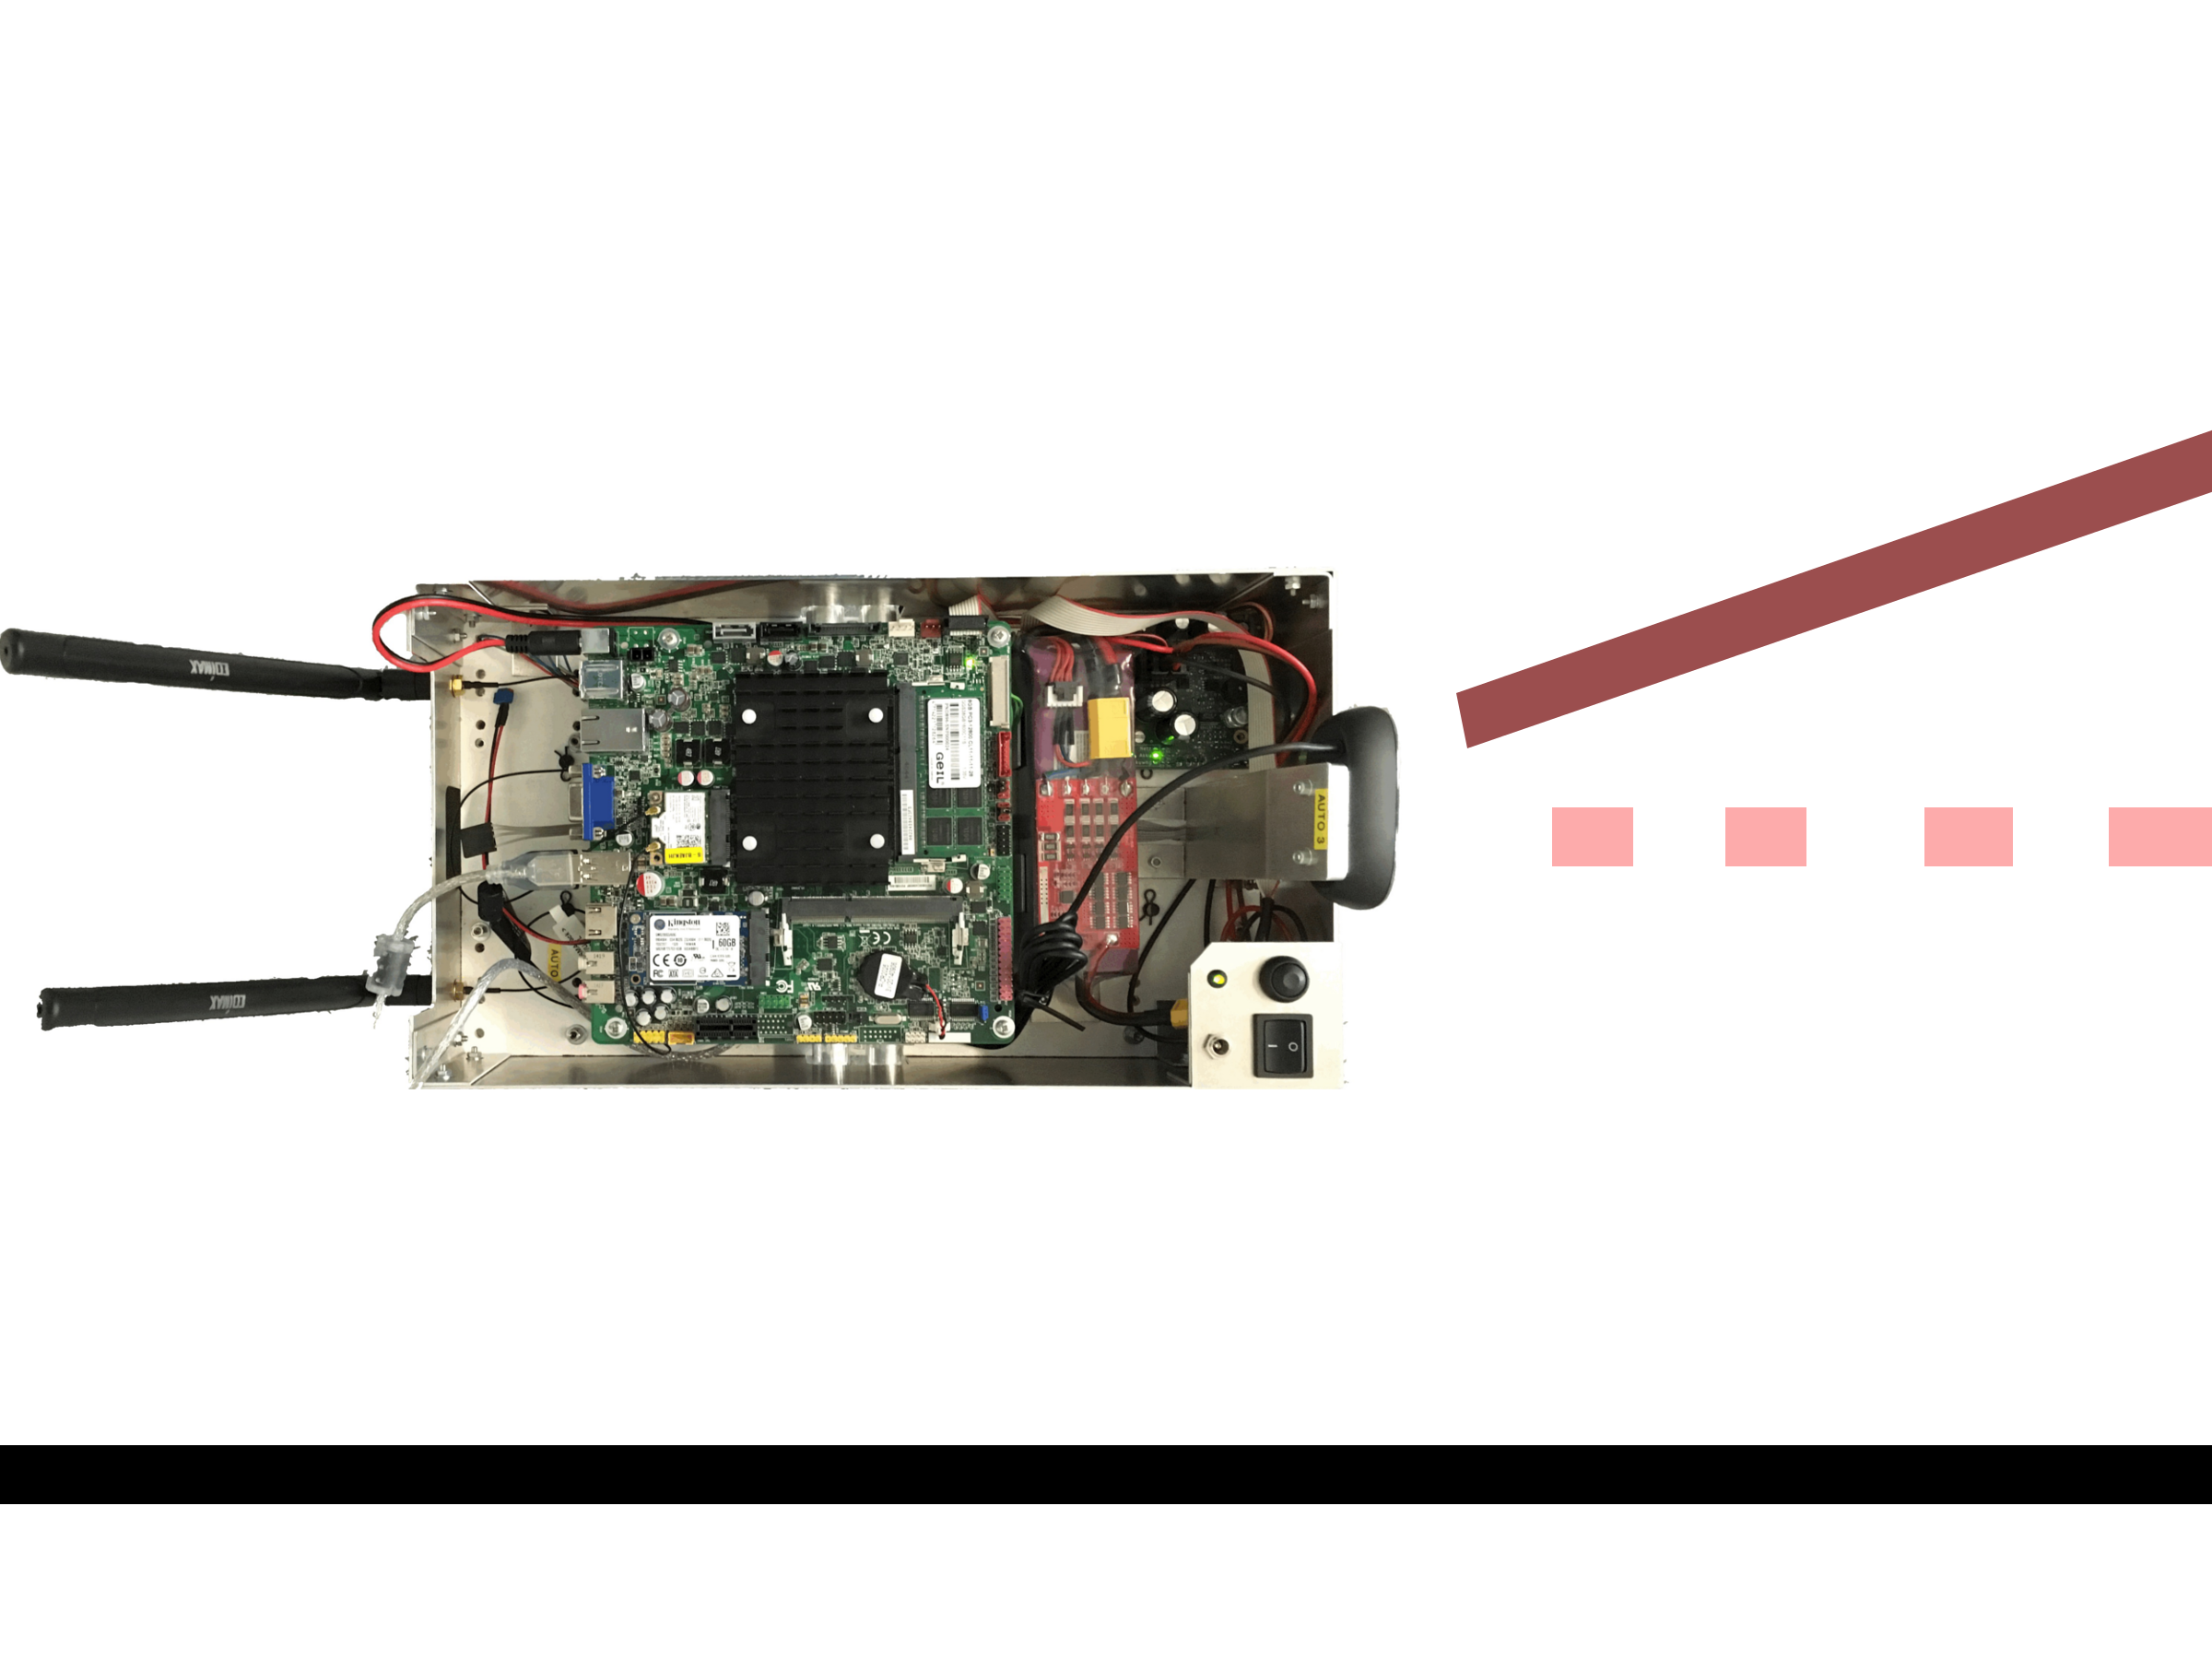
\includegraphics[width=250pt]{images/scharfeRampe.png}
	\caption{Schematische Darstellung des Fahrens einer Rampe}
	\label{fig:ScharfeRampe}
\end{figure}

Diese neue Funktion des Autos wurde nun von uns verwendet, um ein durch die Kamera erkanntes ArUco-Tor, dessen Koordinaten im Raum übergeben wurden, auf einen Punkt einen Meter vor dem Tor anzusteuern.
Weiter oben wurde bereits der Umstand erwähnt, dass es mit einer S-Kurve möglich ist, eine gerade Ausrichtung des Autos zu erreichen. Dies ist mit der Rampenfunktion nicht möglich. Vielmehr ist die Ausrichtung fast nie gleich, da durch die Regelung unterschiedliche Lenkwinkel angenommen werden. In der Regel ist das Auto jedoch in Fahrtrichtung um einen geringen Winkel zwischen $0^\circ$ und $45^\circ$ zur Parallelen zur Wand durch den Tormittelpunkt versetzt. Daher muss die gefeuerte Transition nun noch in zwei weitere Zustände, einen zum Ausrichten des Autos (ArucoGateCenter) und einen zum geradeaus fahren (Motor), überführen. Ersterer macht nichts anderes, als zu prüfen, ob der Tormittelpunkt auf der linken oder rechten Seite des Autos ist und den Lenkeinschlank in entsprechender Richtung auf 1.0 zu setzen und das Auto so weit zu bewegen, bis es ausgerichtet ist. Der Motor-State liest aus seiner JSON-Konfiguration den übergebenen Lenkeinschlag und die Geschwindigkeit und fährt mit dieser Konfiguration so lange, bis die folgende Transition feuert. 
\newline
\newline
Wie man sehen kann, benötigen wir lediglich drei Zustände, um die Tordurchfahrt zu realisieren. Dank unserer FSM-Struktur ist es uns so einfach möglich, z.B. indem das Erkennen und Durchfahren eines ArUco-Tores parallel zu einem anderen Pfad geschaltet wird, flexibel auf auftauchende Tore zu reagieren und diese zu durchfahren. 
  